\graphicspath{{images/analytics/}}
\section{Аналитика}

Раздел \quotes{Аналитика} предназначен для просмотра аналитических сведений о прохождении, 
зачислении и оплате студентами МООК"=курсов. 
Перейти в раздел можно, выбрав его в верхнем меню (см. рис. ~\ref{analytics:top_menu}).

\begin{figure}[H]
	\center{
\includegraphics[width=1\linewidth]{top_menu}}
	\caption{Раздел \quotes{Аналитика}}
	\label{analytics:top_menu}
\end{figure}


Раздел \quotes{Аналитика} содержит следующие типы аналитики:
\begin{itemize}
	\item активность (см.\ подраздел~\ref{analytics:activity});
	\item вовлечённость (см.\ подраздел~\ref{analytics:involvement});
	\item успеваемость (см.\ подраздел~\ref{analytics:progress});
	\item оплата (см.\ подраздел~\ref{analytics:payments});
	\item зачисление (см.\ подраздел~\ref{analytics:enrollment}).
\end{itemize}

Выбор типа аналитики осуществляется с помощью соответствующего элемента формы настройки 
(см.\ подраздел~\ref{analytics:form}).

Аналитические данные каждого типа отображаются в виде графических 
(см.\ подраздел~\ref{analytics:charts}) и табличных данных (см.\ подраздел~\ref{analytics:tables}). 

\subsection{Роли и операции}
Раздел доступен пользователям, имеющим следующие роли:
\begin{itemize}
	\item Администратор вуза, если вуз является поставщиком и потребителем:
	\begin{itemize}
		\item просмотр аналитических сведений о прохождении курсов в рамках вуза.
	\end{itemize}
	\item Администратор вуза, если вуз является только потребителем:
	\begin{itemize}
		\item просмотр аналитических сведений о прохождении курсов студентами своего вуза.
	\end{itemize}
	\item Автор курса:
	\begin{itemize}
		\item просмотр аналитических сведений о прохождении своих курсов.
	\end{itemize}
\end{itemize}

\subsection{Форма настройки}
\label{analytics:form}

Форма настройки отображения аналитики позволяет выбрать тип, детализацию и произвести фильтрацию
аналитических данных. Общий вид формы приведён на рис.~\ref{analytics:form:pic}

\begin{figure}[H]
	\center{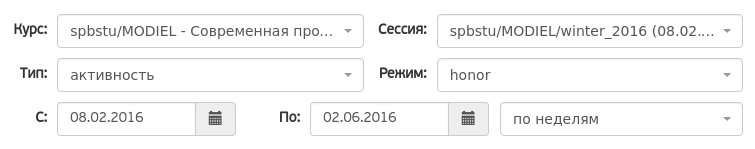
\includegraphics[width=1\linewidth]{analytics_form}}
	\caption{Форма настройки аналитики}
	\label{analytics:form:pic}
\end{figure}

Форма содержит следующие элементы:
\begin{itemize}
	\item Выбор курса "--- выпадающий список курсов с автодополнением (см.\ подраздел~\ref{widget:autocomplete}).
	Автодополнение происходит по следующим полям курса:
	\begin{itemize}
	 	\item название курса;
	 	\item код университета;
	 	\item код курса.
	 \end{itemize}
	\item Выбор сессии курса "--- выпадающий список курсов с автодополнением (см.\ подраздел~\ref{widget:autocomplete}).
	При выборе другого курса или при загрузке страницы выбирается текущая или (если таковой нет) последняя
	сессия выбранного курса. Автодополнение происходит по коду сессии курса.
	\item Выбор типа аналитики "--- выпадающий список.
	\item Фильтрация по режиму прохождения курса. Режим \quotes{all} отображает данные по всем режимам.
	\item Фильтрация по дате "--- два элемента для выбора даты начала и конца интервала отображения (см.\ подраздел~\ref{widget:date_time_picker})
	При выборе курса, сессии курса или при загрузке страницы даты устанавливаются в дату начала и конца выбранной сессии.
	\item Выбор детализации "--- выпадающий список. Доступны следующие степени детализации:
	\begin{itemize}
		\item по дням;
		\item по неделям (по умолчанию);
		\item по месяцам.
	\end{itemize}
\end{itemize}

Доступные для выбора курсы и сессии зависят от прав конкретного пользователя.
\begin{itemize}
	\item Администратору вуза, являющегося поставщиком и потребителем, доступны курсы и сессии текущего вуза.
	\item Администратору вуза, являющегося только потребителем, доступны курсы и сессии курсов, на которых 
	обучаются студенты текущего вуза. Аналитические данные для чужих курсов отфильтрованы по текущему вузу.
	\item Автору курса доступны курсы, автором которых он является и сессии этих курсов.
\end{itemize}


При изменении значений какого-либо из полей формы аналитические данные на странице обновляются автоматически.

\subsection{Графики}
\label{analytics:charts}

Для всех видов аналитики кроме успеваемости (описание графика успеваемости см. в подразделе~\ref{analytics:progress}) 
графики представляют собой двумерные линейные графики с одной или несколькими линиями. Пример графика
приведён на рис.~\ref{analytics:chart}. По оси абсцисс отложены интервалы дат (в случае 
детализации по дням "--- даты), по оси ординат "--- значения отображаемых величин. 

\begin{figure}[H]
	\center{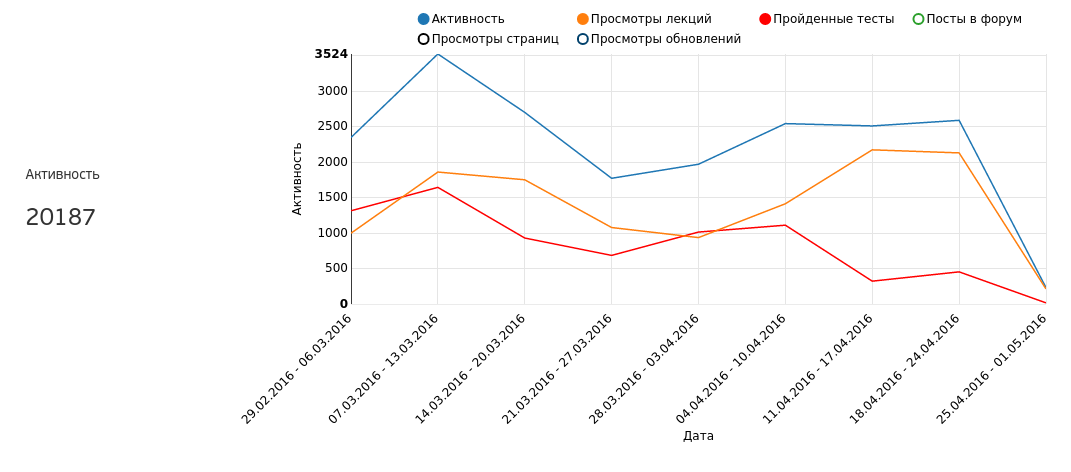
\includegraphics[width=1\linewidth]{analytics_chart}}
	\caption{Пример графика аналитики}
	\label{analytics:chart}
\end{figure}

Слева от графиков расположены значения суммарных показателей по временному интервалу для выбранного 
типа аналитики.\footnote{Кроме зачисления, см.\ подраздел~\ref{analytics:enrollment}}

Над графиком расположена интерактивная легенда, позволяющая включать и отключать отображение отдельных линий
графика (в случае наличия нескольких линий на графике).
\begin{itemize}
	\item Для включения или отключения определённой линии графика следует нажать на соответствующий пункт легенды.
	\item Для того, чтобы оставить на графике только одну выбранную линию следует дважды нажать на соответствующий пункт легенды.
	\item В случае, если на графике осталась только одна линия, при попытке отключения её отображения будет включено отображение всех линий. 
\end{itemize}
По умолчанию показывается только основной график для выбранного типа аналитики.

При перемещении курсора мыши по графику, на графике появляются интерактивные подсказки, показывающие
значение абсциссы в данной точке и значения ординат для каждой отображаемой линии (см.\ рис.~\ref{analytics:chart:tooltip}.

\begin{figure}[H]
	\center{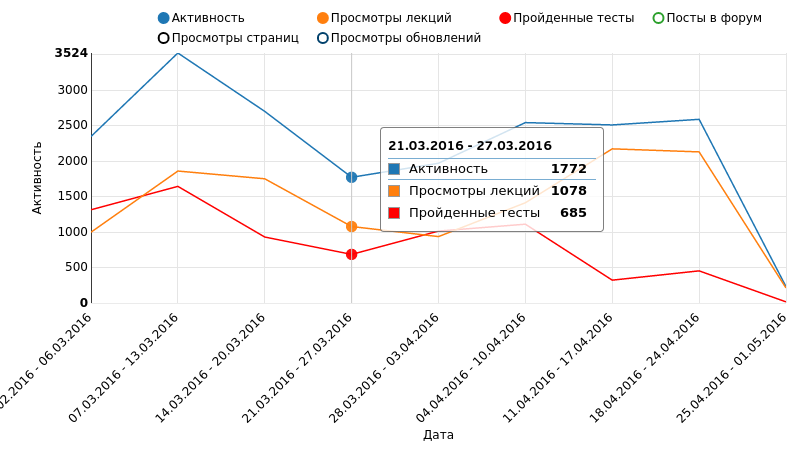
\includegraphics[width=1\linewidth]{analytics_chart_tooltip}}
	\caption{Пример всплывающей подсказки на графике аналитики}
	\label{analytics:chart:tooltip}
\end{figure}

\subsection{Табличные данные}
\label{analytics:tables}

Для всех видов аналитики кроме успеваемости (описание графика успеваемости см. в подразделе~\ref{analytics:progress})
в таблице отображены те же данные, что и на графике. 
Описание элементов управления таблицей см.\ в подразделе~\ref{sec:datatables}. Также в данном разделе описан механизм
сортировки данных в таблице. 

В первом столбце таблицы содержится интервал времени (ось абсцисс на графике), для которого в 
остальных столбцах отображены значения параметров (ось ординат на графике).

Общий вид таблиц показан на рис.~\ref{analytics:table}

\begin{figure}[H]
	\center{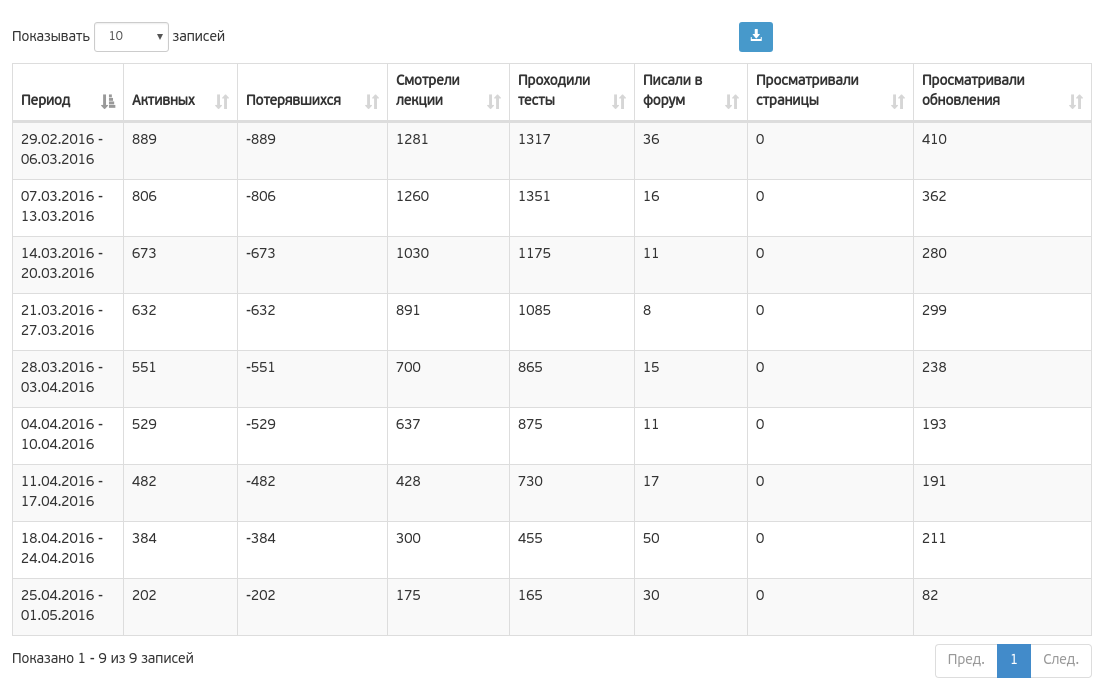
\includegraphics[width=1\linewidth]{analytics_table}}
	\caption{Пример таблицы аналитики}
	\label{analytics:table}
\end{figure}

\subsection{Активность}
\label{analytics:activity}

Для типа аналитики \quotes{Активность} отображаются следующие значения:
\begin{itemize}
	\item активность (основной показатель для данного типа аналитики);
	\item просмотры лекций;
	\item пройденные тесты;
	\item посты в форум;
	\item просмотры страниц;
	\item просмотры обновлений.
\end{itemize}

Отображение и элементы управления графических и табличных данных соответствуют описанию в 
подразделах~\ref{analytics:charts}--\ref{analytics:tables}.

\subsection{Вовлечённость}
\label{analytics:involvement}

Для типа аналитики \quotes{Вовлечённость} отображаются следующие значения:
\begin{itemize}
	\item число активных студентов (основной показатель для данного типа аналитики);
	\item число потерявшихся студентов;
	\item число студентов, смотревших лекции;
	\item число студентов, проходивших тесты;
	\item число студентов, писавших в форум;
	\item число студентов, просматривавших страницы курса;
	\item число студентов, просматривавших обновления курса.
\end{itemize}

Отображение и элементы управления графических и табличных данных соответствуют описанию в 
подразделах~\ref{analytics:charts}--\ref{analytics:tables}.

\subsection{Оплата}
\label{analytics:payments}
Для типа аналитики \quotes{Оплата} отображается сумма платежей за период времени (точку на оси абсцисс).

Отображение и элементы управления графических и табличных данных соответствуют описанию в 
подразделах~\ref{analytics:charts}--\ref{analytics:tables}.

\subsection{Зачисление}
\label{analytics:enrollment}

Для типа аналитики \quotes{Зачисление} отображаются количество студентов, которые были зачислены на курс к 
моменту окончания интервала (точки на оси абсцисс).

Отображение и элементы управления графических и табличных данных в целом соответствуют описанию в 
подразделах~\ref{analytics:charts}--\ref{analytics:tables}. В левой части графика показано число
студентов, зачисленных к концу последнего интервала на графике.

\subsection{Успеваемость}
\label{analytics:progress}

Отображение типа аналитики \quotes{Успеваемость} также содержит график и таблицу, но значительно
отличается от других типов. В режиме \quotes{Успеваемость} в форме настроек недоступны фильтры
по временному интервалу и настройки детализации. Далее описаны график и таблица режима \quotes{Успеваемость}.

\subsubsection{График}

График успеваемости представляет собой столбчатую диаграмму. 
Общий вид графика успеваемости показан на рис.~\ref{analytics:progress:chart}.


\begin{figure}[H]
	\center{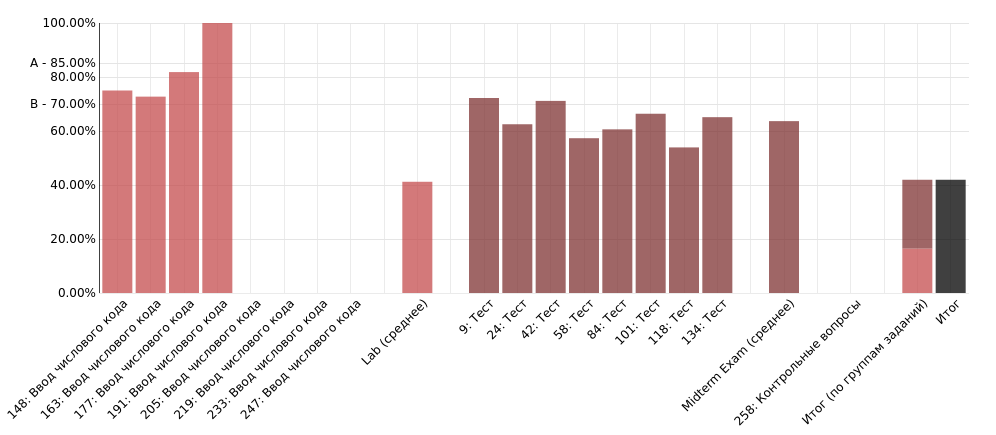
\includegraphics[width=1\linewidth]{analytics_progress_chart}}
	\caption{График успеваемости}
	\label{analytics:progress:chart}
\end{figure}

По оси абсцисс отложены задания текущего курса. По оси ординат "--- средний результат студентов 
(с учётом фильтрации по вузу) по текущему заданию.

Задания сгруппированы в соответствии с группами, заданными автором курса в LCMS.
Группировка осуществляется по цветам и с помощью пространственного разделения.
В случае, если в группе несколько заданий, справа от столбцов отдельных заданий добавляется столбец 
среднего результата по группе (данный столбец отмечен меткой на оси абсцисс). Предпоследний столбец 
"--- общий средний итог по группам заданий. Данный столбец содержит один или несколько вертикальных слоёв,
каждый из которых соответствует группе заданий. В высоте слоёв учтён вес данной группы, 
заданный в LCMS. Последний столбец "--- общий средний итог студентов по данному курсу. Высота его
равна высоте предыдущего столбца, отличается лишь всплывающая подсказка.

На оси ординат отложен средний результат студентов по заданиям в процентах. На этой оси присутствуют метки,
кратные 20\% (\quotes{чётные} метки), а также метки оценок, заданные в LCMS (с названием оценки). 
В случае близости метки оценки и \quotes{чётной} метки, чётная метка скрывается.

При перемещении курсора мыши по графику, на графике появляются интерактивные подсказки.
Для отдельных заданий и средних значений по группам заданий в подсказке показана метка оси абсцисс
и средний результат студентов по данному заданию или группе (см.\ рис.~\ref{analytics:progress:chart:tooltip:individual}).
Для столбца с итогом по группам заданий для каждого вертикального слоя показывается подсказка
с названием группы заданий и её вкладом (в процентах) в общий итог (см.\ рис.~\ref{analytics:progress:chart:tooltip:avg_group}).
Для столбца с общим итогом показывается подсказка
с общим итогом в процентах (см.\ рис.~\ref{analytics:progress:chart:tooltip:avg_group}).


\begin{figure}[H]
	\center{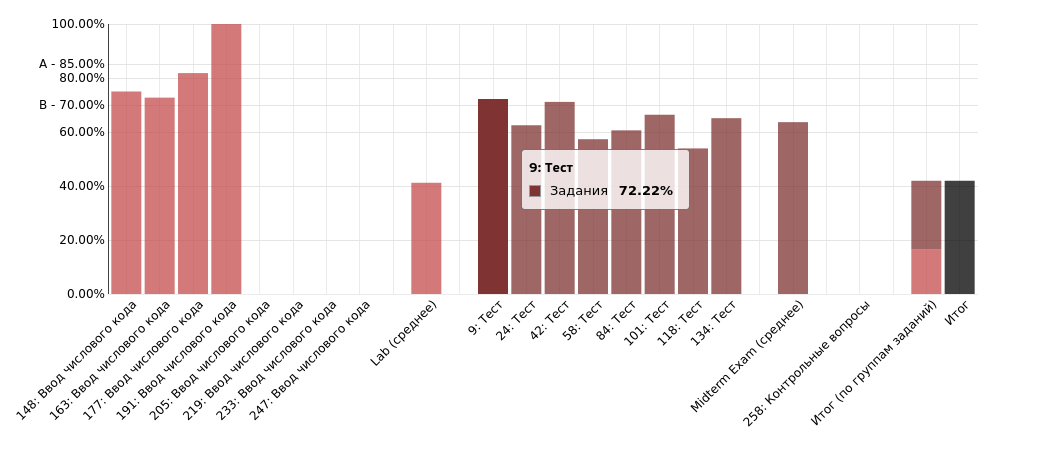
\includegraphics[width=1\linewidth]{analytics_progress_chart_tooltip_individual}}
	\caption{Всплывающая подсказка для задания на графике успеваемости}
	\label{analytics:progress:chart:tooltip:individual}
\end{figure}


\begin{figure}[H]
	\center{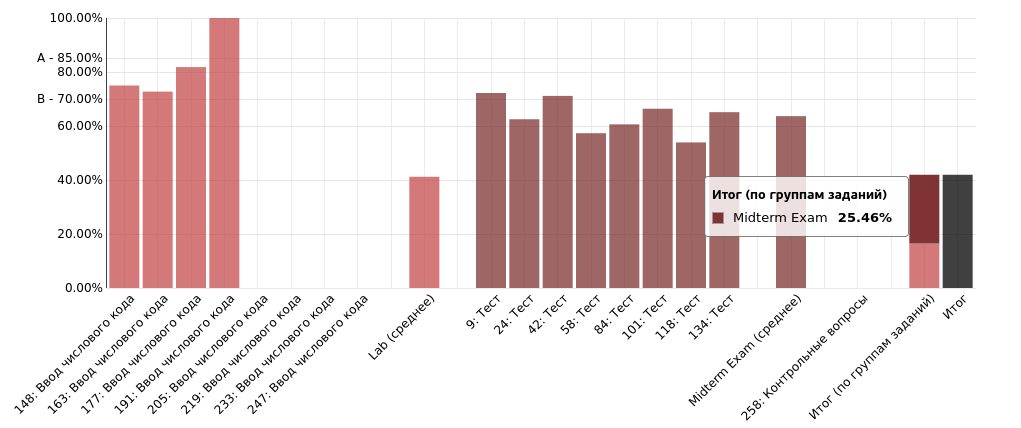
\includegraphics[width=1\linewidth]{analytics_progress_chart_tooltip_avg_group}}
	\caption{Всплывающая подсказка для столбца с итогом по группам заданий на графике успеваемости}
	\label{analytics:progress:chart:tooltip:avg_group}
\end{figure}


\begin{figure}[H]
	\center{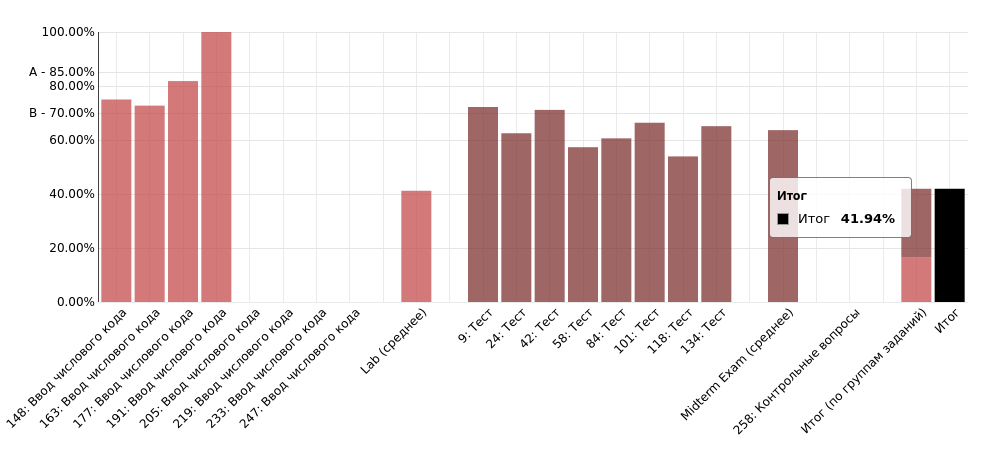
\includegraphics[width=1\linewidth]{analytics_progress_chart_tooltip_avg}}
	\caption{Всплывающая подсказка для столбца с итогом на графике успеваемости}
	\label{analytics:progress:chart:tooltip:avg}
\end{figure}

\subsubsection{Таблица}

Таблица содержит:
\begin{itemize}
	\item переключатель страниц;
 	\item переключатель количества записей на странице;
 	\item кнопку \quotes{CSV} для выгрузки табличных данных в 
 	CSV \footnote{Выгрузка всегда происходит в синхронном режиме};
 	\item полосу горизонтальной прокрутки (первый и два последний столбца всегда видимы).
\end{itemize} 
Описание данных элементов см.\ в подразделе~\ref{sec:datatables}. Также в данном разделе описан механизм
сортировки данных в таблице. 


В отличие от других разделов аналитики, строка таблицы не соответствует точке на графике. 
В каждой строке содержится успеваемость каждого студента.
\begin{itemize}
	\item первый столбец "--- ФИО студента;
	\item предпоследний столбец "--- общий итог студента;
	\item последний столбец "--- оценка студента (если результат студента больше минимальной оценки за курс)
	\footnote{При сортировке по данному столбцу фактически происходит сортировка по общему итогу 
	студента (а не алфавитная сортировка по оценкам)}
\end{itemize}
Остальные столбцы соответствуют столбцам на графике, но отображают индивидуальные данные для 
каждого студента.

Общий вид таблицы приведён на рис.~\ref{analytics:progress:table}
\begin{figure}[H]
	\center{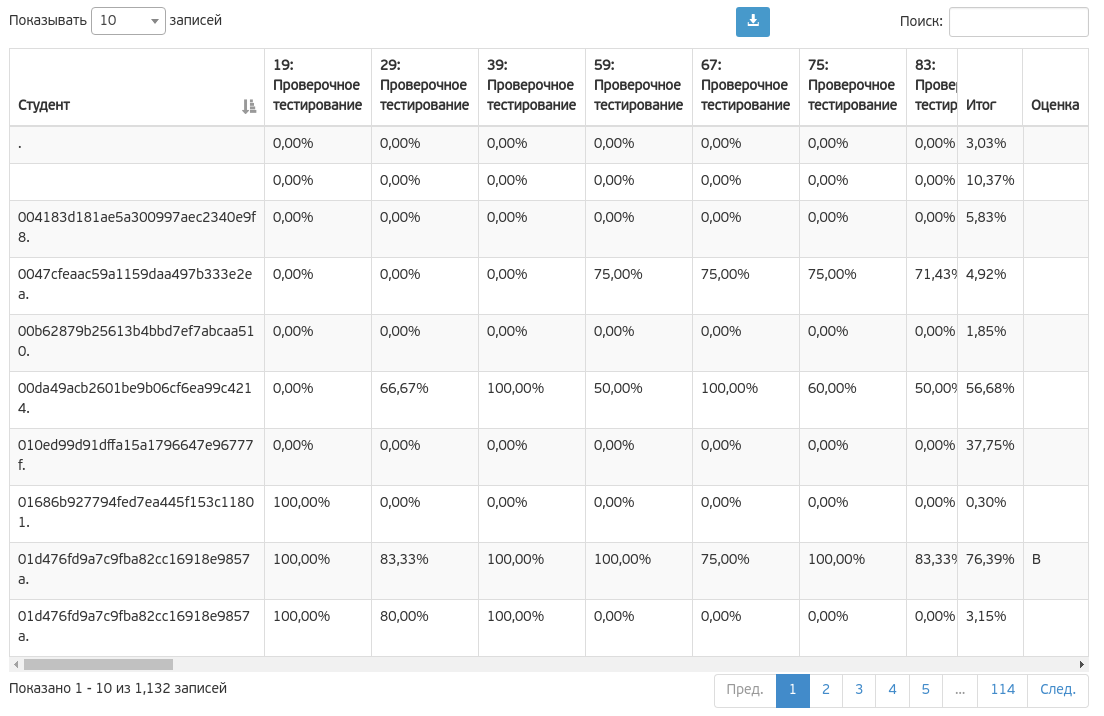
\includegraphics[width=1\linewidth]{progress_table}}
	\caption{Таблица успеваемости}
	\label{analytics:progress:table}
\end{figure}